\section{File-level redundant ratio}
\label{sec:dedup}

\subsection{Overview of redundant file overhead in terms of file repeat count and redundant storage overhead}

\begin{figure}
	\centering
	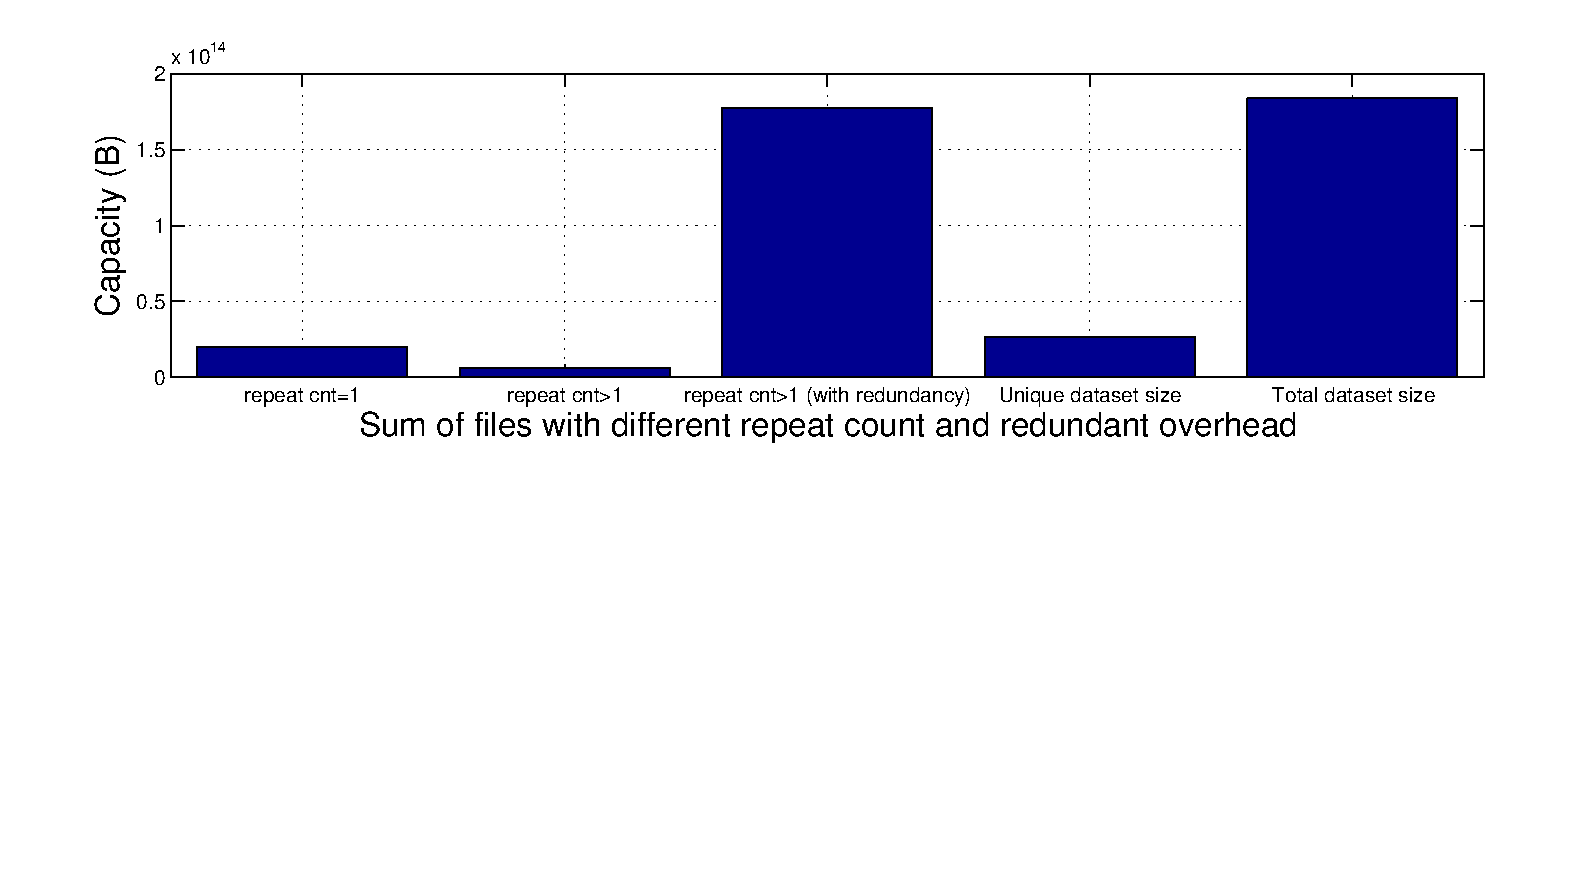
\includegraphics[width=0.5\textwidth]{graphs/capacity_data_ratio.eps}
	\caption{Redundant storage overhead.
	}
	\label{fig_redundant_overhead}
\end{figure}

\begin{table} 
	\centering 
	\scriptsize  
	%\begin{minipage}{.5\linewidth}
	\caption{Redundant ratio in terms of file count and capacity} \label{tbl:redundant_ratio} 
	\begin{tabular}{|l|l|l|}%p{0.14\textwidth} 
		\hline 
		% after \\: \hline or \cline{col1-col2} \cline{col3-col4} ... 
		% after \\: \hline or \cline{col1-col2} \cline{col3-col4} ... 
		       & File count & Capacity \\
		\hline
		Repeat cnt = 1 & 0.58\% & 10.87\%\\
		\hline
		Repeat cnt $>$ 1 after dedup & 2.59\% & 3.44\%\\
		\hline
		Repeat cnt $>$ 1 before dedup  & 99.42\%  & 89.13\%\\
		\hline
		Unique dataset (Uncompressed) & 3.17\% (167,251,437)  &  14.31\% (23.92 TB) \\
		\hline 
		Total dataset (Uncompressed) & 5,278,465,130 & 167.20 TB \\
		\hline 	
		%\hline 
	\end{tabular} 
\end{table} 

\subsection{Redundant ratio for layers}

\subsubsection{Overview of redundant ratio for layers in terms of per-layer redundant ratio and across-layer redundant ratio}

\paragraph{Per-layer redundant ratio} Per-layer redundant ratio is shown in Table~\ref{tbl:per_ratio_layers}.

\begin{table} 
	\centering 
	\scriptsize  
	%\begin{minipage}{.5\linewidth}
	\caption{Per-layer redundant ratio for layers in terms of file count and capacity} \label{tbl:per_ratio_layers} 
	\begin{tabular}{|l|l|l|}%p{0.14\textwidth} 
		\hline 
		% after \\: \hline or \cline{col1-col2} \cline{col3-col4} ... 
		% after \\: \hline or \cline{col1-col2} \cline{col3-col4} ... 
		& File count & Capacity \\
		\hline
		Avg. & 49.78\% & -\\
		\hline
		Median & - & - \\
		\hline
		Max. & 100\% & -\\
		\hline
		Min.  & 0.00\%  & -\\
		\hline
		Stdev.  &  2.14\% & -\\
		\hline
		Layer dataset after Red.-dedup (Uncompressed) & -  & -\\
		\hline 
		Total layer dataset (Uncompressed) &  -	& -\\
		\hline 
		%\hline 
	\end{tabular} 
\end{table}

\paragraph{Across-layer redundant ratio} Across-layer redundant ratio is shown in Table~\ref{tbl:across_ratio_layers}

\begin{table} 
	\centering 
	\scriptsize  
	%\begin{minipage}{.5\linewidth}
	\caption{Across-layer redundant ratio for layers in terms of file count and capacity} \label{tbl:across_ratio_layers} 
	\begin{tabular}{|l|l|l|}%p{0.14\textwidth} 
		\hline 
		% after \\: \hline or \cline{col1-col2} \cline{col3-col4} ... 
		% after \\: \hline or \cline{col1-col2} \cline{col3-col4} ... 
		& File count & Capacity \\
		\hline
		Avg. & 98.75\% & -\\
		\hline
		Median & - & - \\
		\hline
		Max. & 1 & -\\
		\hline
		Min.  & 0.87\%  & -\\
		\hline
		Stdev.  &  4.70\% & -\\
		\hline
		Layer dataset after share.-dedup (Uncompressed) & -  & -\\
		\hline 
		Total layer dataset (Uncompressed) &  -	& -\\
		\hline
	\end{tabular} 
\end{table}

\subsubsection{Per-layer redundant overhead}

\paragraph{Cumulative distribution and probability distribution of per-layer redundant ratio in terms of file count and storage capacity}

\begin{figure}
	\centering
	%\includegraphics [width=0.45\textwidth]{plots/exp-total-stev-erase.eps}
	\subfigure[CDF of per-layer redundant ratio in terms of file count]{\label{fig:per_layer_ratio_fcnt_cdf}
		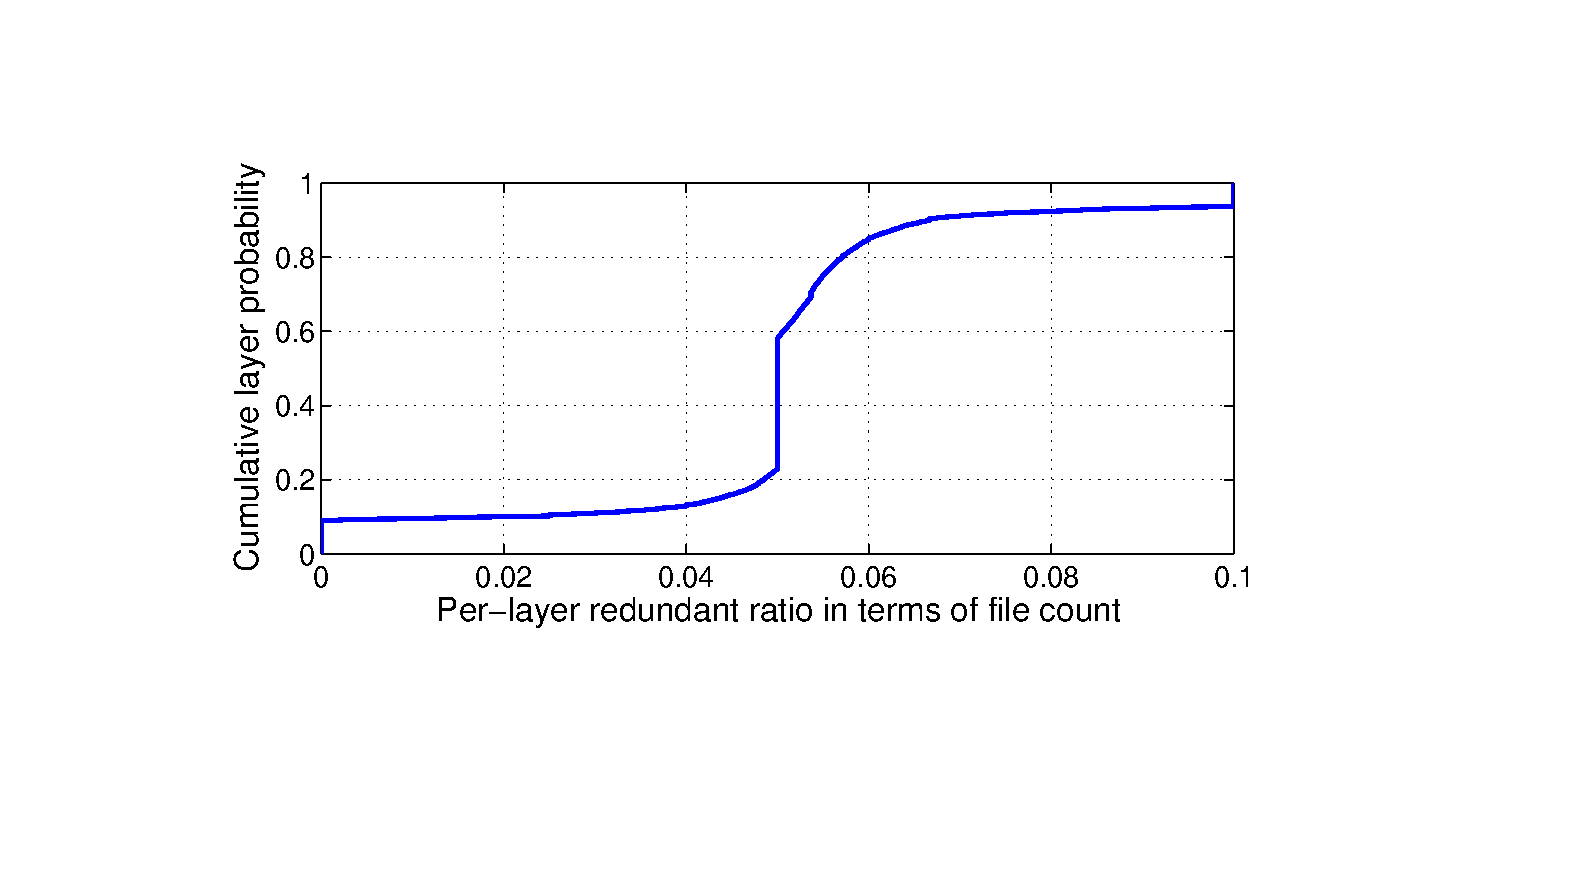
\includegraphics [width=0.5\textwidth]{graphs/per_layer_ratio_fcnt_cdf.eps}
	}
	\subfigure[PDF of per-layer redundant ratio in terms of file count]{\label{fig:per_layer_ratio_fcnt_pdf}
		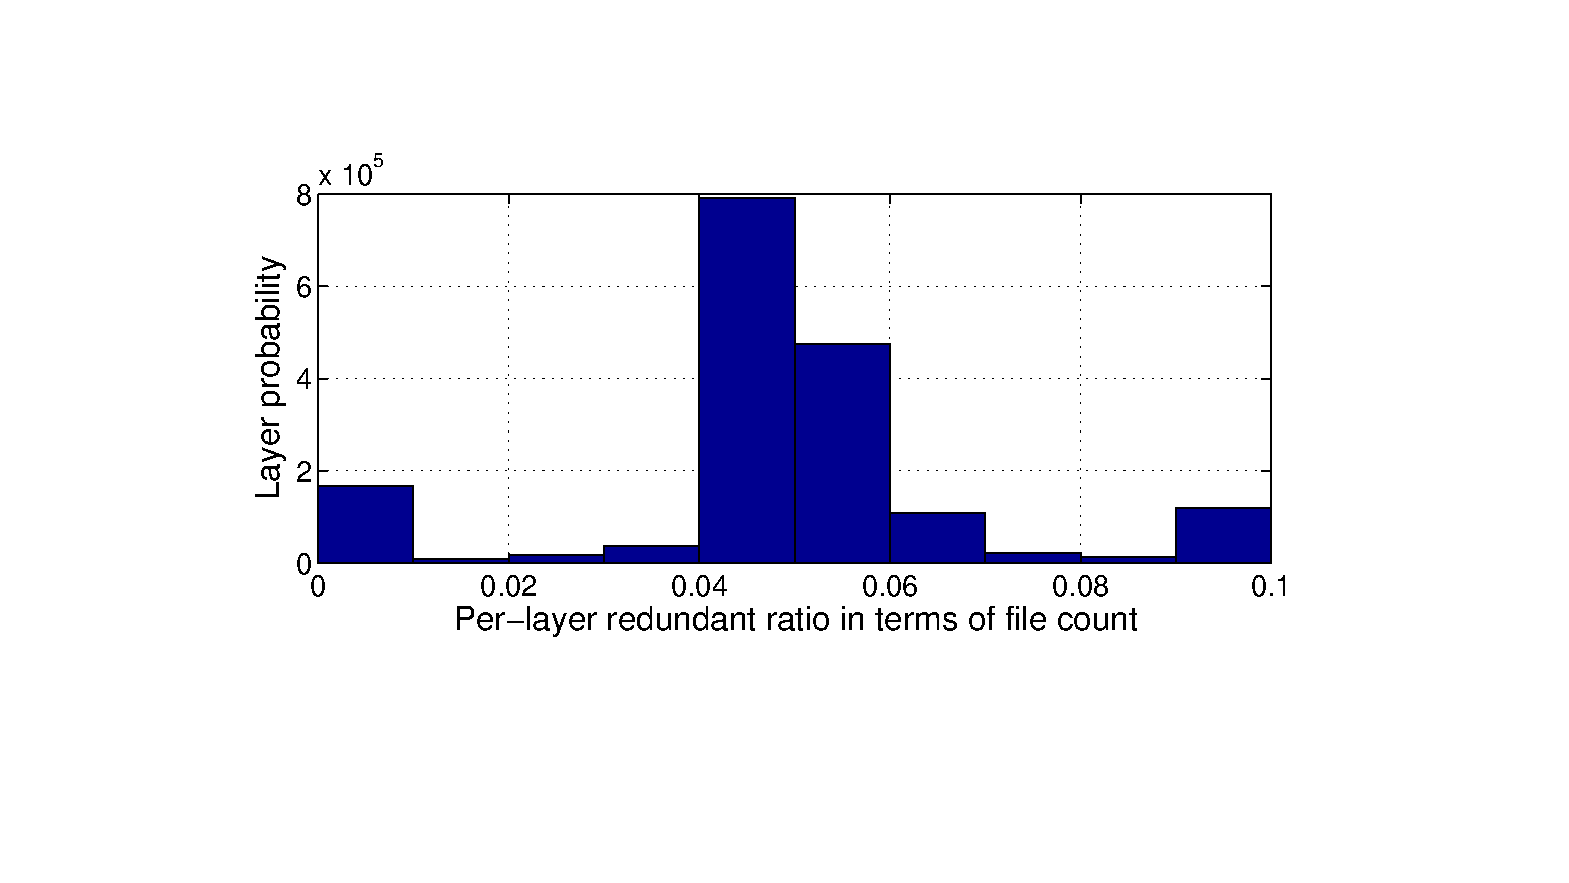
\includegraphics [width=0.5\textwidth]{graphs/per_layer_ratio_fcnt_pdf.eps}
	}
	\caption{Wear variance}
	\label{fig:eval-stdev-erasure-cnt}
\end{figure}

\paragraph{Per-layer redundant ratio by layer size in terms of file count and storage capacity}

\subsubsection{Across-layer redundant overhead}

\paragraph{Cumulative distribution and probability distribution of across-layer redundant ratio in terms of file count and storage capacity}

\begin{figure}
	\centering
	%\includegraphics [width=0.45\textwidth]{plots/exp-total-stev-erase.eps}
	\subfigure[CDF of across-layer redundant ratio in terms of file count]{\label{fig:across_layer_ratio_fcnt_cdf}
		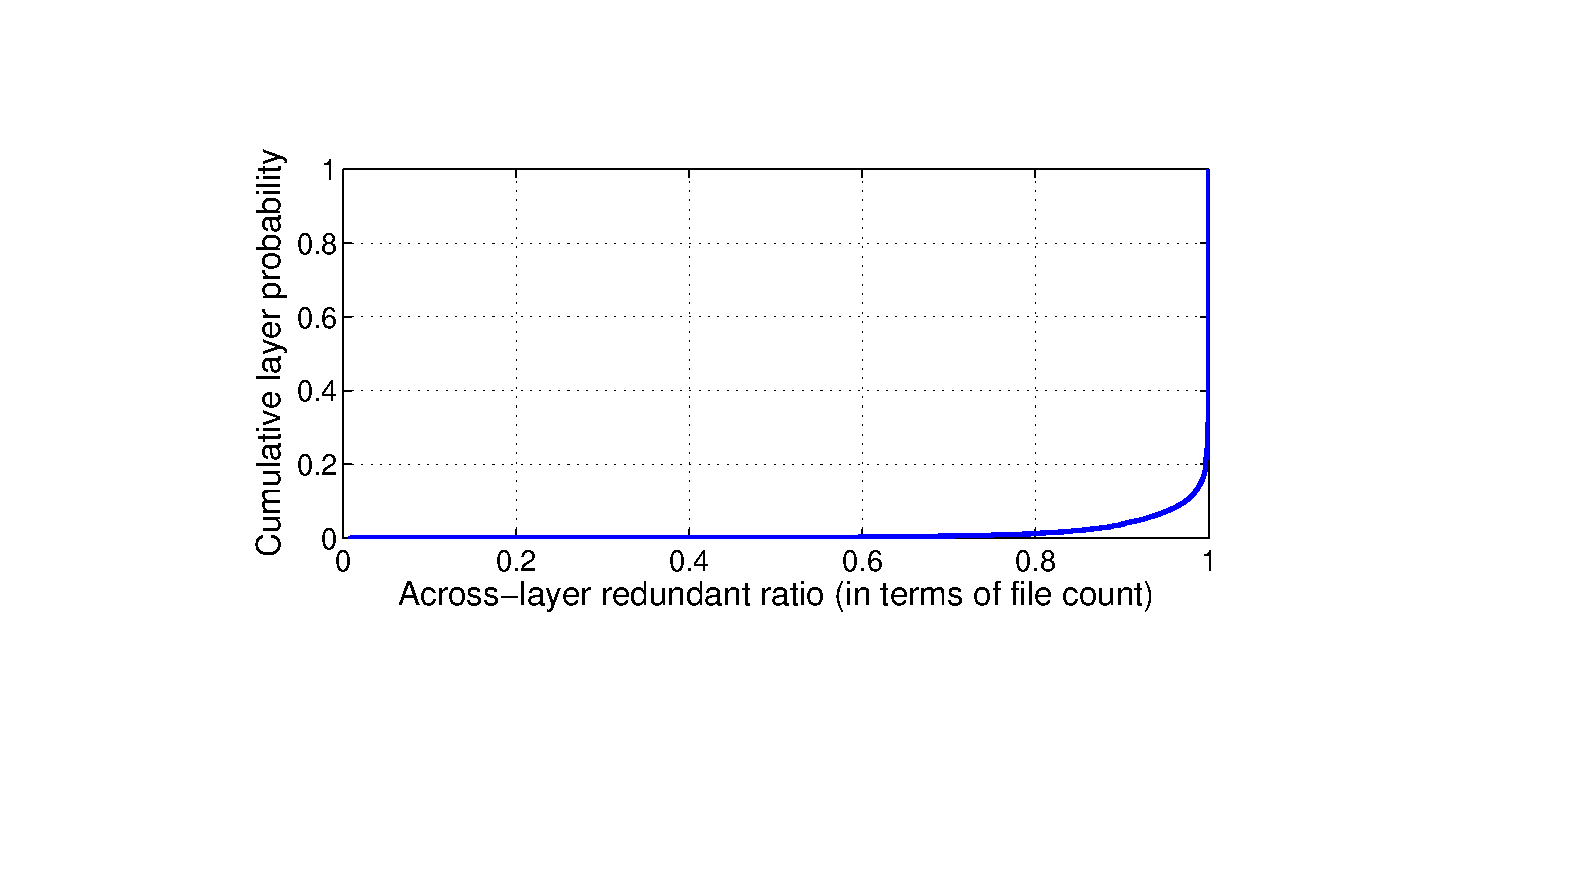
\includegraphics [width=0.5\textwidth]{graphs/across_layer_ratio_fcnt_cdf.eps}
	}
	\subfigure[PDF of across-layer redundant ratio in terms of file count]{\label{fig:across_layer_ratio_fcnt_pdf}
		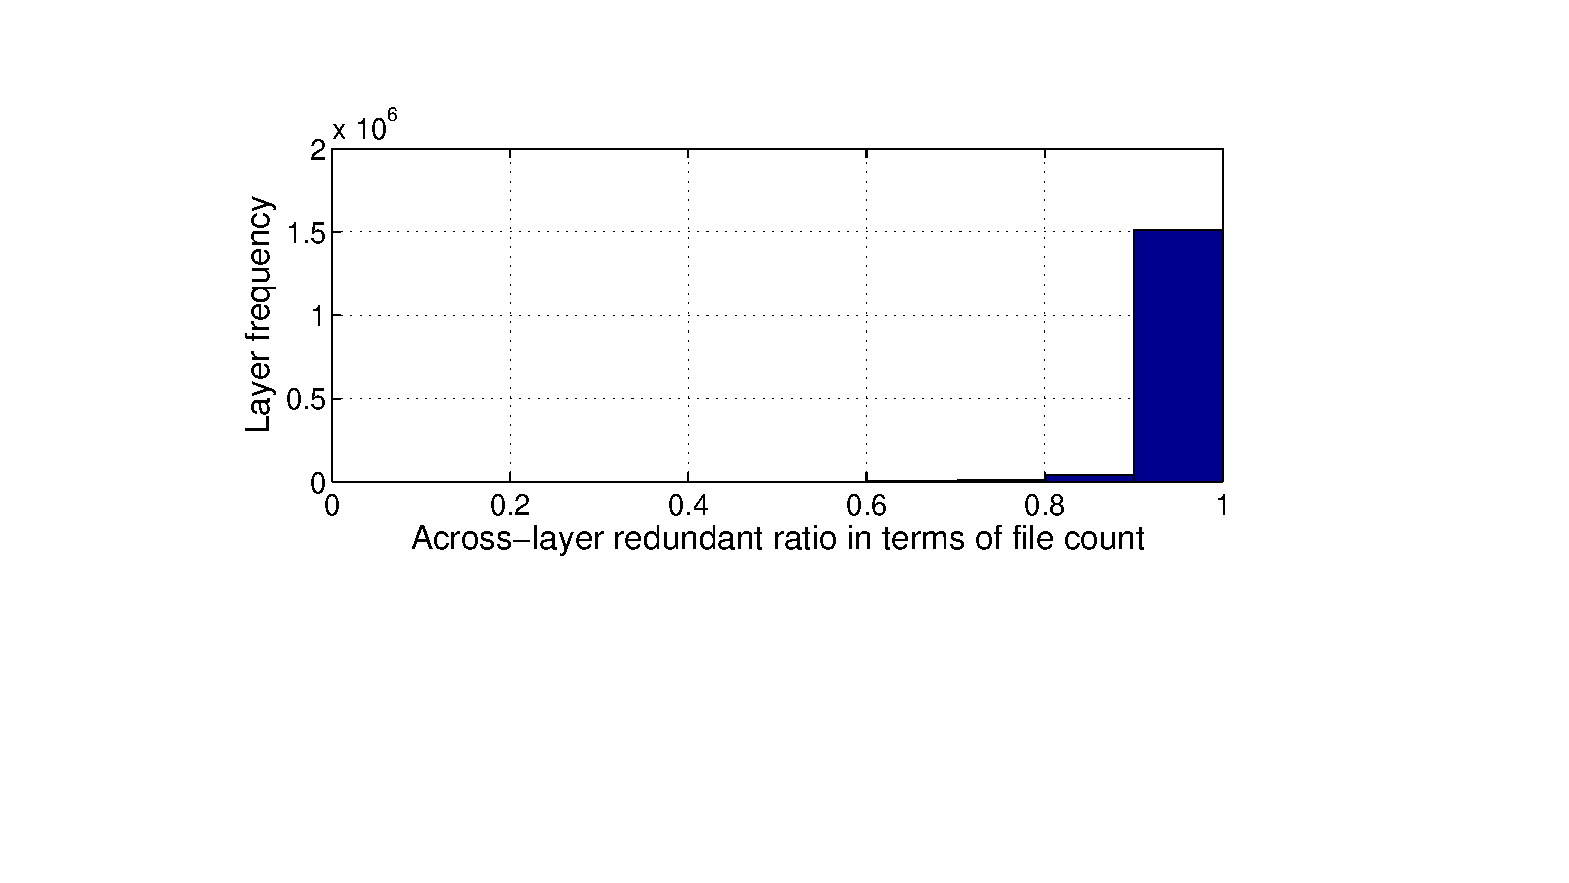
\includegraphics [width=0.5\textwidth]{graphs/across_layer_ratio_fcnt_pdf.eps}
	}
	\caption{Wear variance}
	\label{fig:eval-stdev-erasure-cnt}
\end{figure}

\paragraph{Across-layer redundant ratio by layer size in terms of file count and storage capacity}

\subsection{Redundant ratio for images}

